\documentclass[../main.tex]{subfiles}
\usepackage[utf8]{inputenc}
\usepackage[T1]{fontenc}
\usepackage{graphicx}
\usepackage{longtable}
\usepackage{wrapfig}
\usepackage{rotating}
\usepackage[normalem]{ulem}
\usepackage{amsmath}
\usepackage{amssymb}
\usepackage{capt-of}
\usepackage{hyperref}
\usepackage{float}
\graphicspath{{../}}
\author{Cezary Wieczorkowski}
\date{\today}
\title{Finn}
\hypersetup{
 pdfauthor={Cezary Wieczorkowski},
 pdftitle={Finn},
 pdfkeywords={},
 pdfsubject={},
 pdflang={Polish}}
\begin{document}


\section{Finn}

Finn to narzędzie stworzone przez firmę Xilinx \cite{finn} w celu syntezy oraz implementacji skwantyzowanych sieci neuronowych na układach FPGA. Finn to kolekcja bibliotek które pozwalają użytkownikowi dokonać szeregu
transformacji na wybranej sieci neuronowej tak aby była ona możliwa do zaimplementowania w układzie FPGA. Konkretne transformacje oraz kroki przez które należy przejść zależą od struktury danej sieci neuronowej.

\begin{figure}[H]
    \centering
    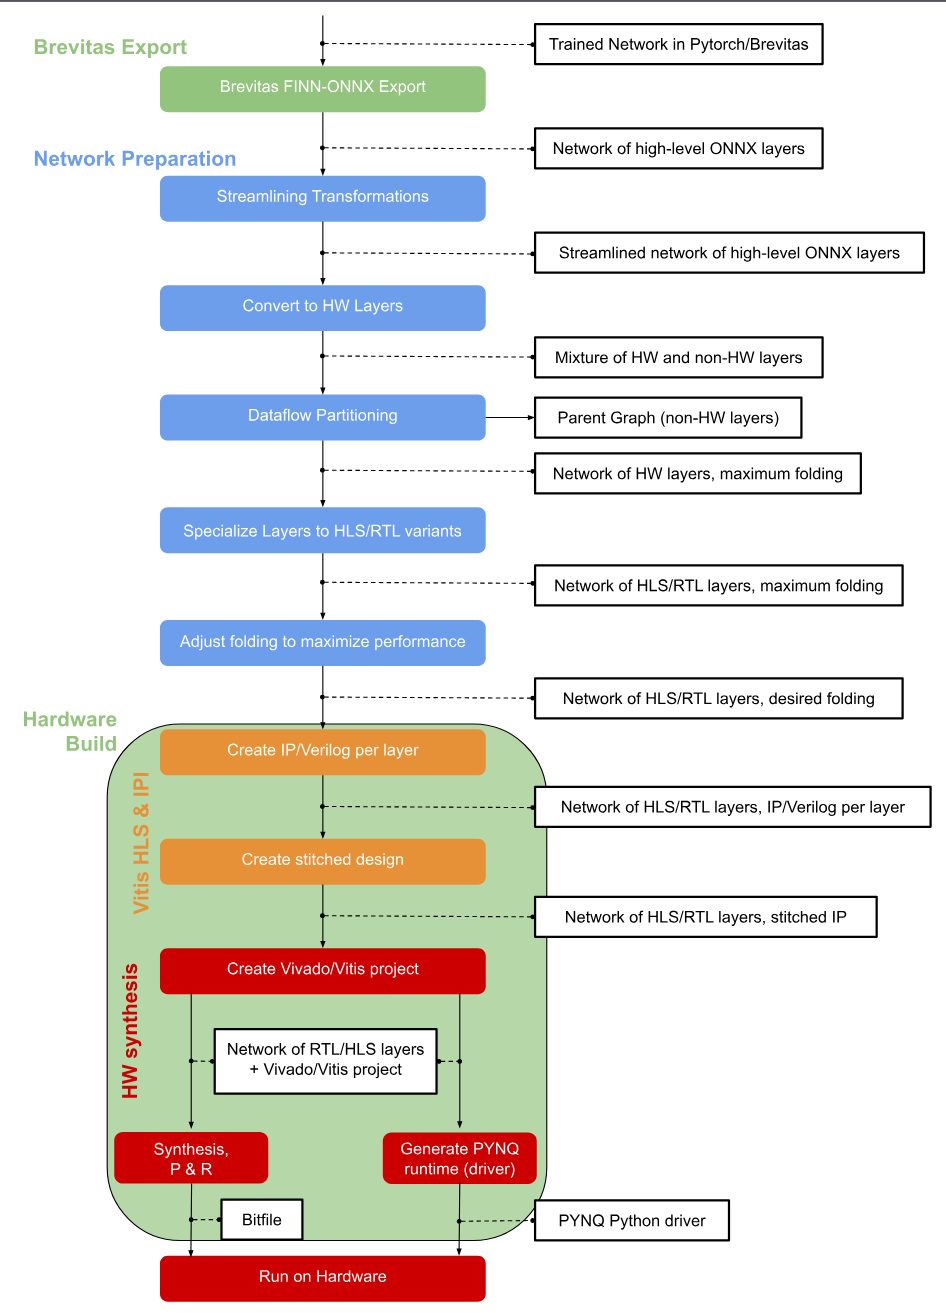
\includegraphics[scale=0.4]{finn_design_flow.png}
    \caption{Etapy implementacji sieci neuronowej przy pomocy Finn}
    \label{fig:finn_flow}
\end{figure}

Standardowy proces implementacji sieci przy pomocy Finn można zobaczyć na \ref{fig:finn_flow}. Pierwszym krokiem jest import modelu w formacie ONNX - jest to otwarty standard uniwersalnej reprezentacji modeli uczenia maszynowego
\cite{onnxruntime}. Biblioteka Brevitas wspiera eksport wytrenowanych modeli do formatu ONNX.

\subsection{Transformacja sieci}

Zaimportowany model musi zostać dostosowany do architektury oraz możliwości biblioteki Finn. Dokonuje się tego poprzez wykonywanie funkcji zwanych transformacjami. W bibliotece Finn dostępne są następujące:

\begin{itemize}
    \item Ogólne - są to transformacje służące do nadawania warstwom nazw lub dedukcji rozmiarów wyjścia warstwy.
    \item Optymalizacyjne - te transformacje zmieniają strukture modelu. Reorganizują warstwy oraz scalają je razem.
    \item HLS - w końcowej fazie przetwarzania modelu powstałe w wyniku uprzednich transformacji warstwy konwertowane są na bloki HLS.
\end{itemize}

Etap transformacji optymalizacyjnych jest kluczowy ze względu na pewne ograniczenia Finn. Model musi zostać zredukowany w taki sposób aby pozostały w nim tylko 
warstwy wykonujące operacje które są możliwe do konwersji na moduły znajdujące się w zasobach bibliotek finn-hls oraz finn-rtl. Typy warstw możliwe do implementacji w sprzęcie przez Finn to:

\begin{itemize}
    \item Mul 
    \item Add
    \item MathMul
    \item MultiThreshold
    \item Im2Co
    \item MaxPoolNWHC
\end{itemize}

Ponadto wejście każdej z warstw musi być liczbą całkowitą - jest to jedyny typ danych wspierany przez implementacje sprzętowe biblioteki Finn.

\subsection{Generacja implementacji sprzętowej}

Etap generacji sprzętowej odpowiada za przeprowadzenie syntezy oraz implementacji sieci neuronowej do akceleratora który można wgrać na układ FPGA. Proces budowania jest wywoływany 
jako kolejna transformacja modelu:

\begin{minted}{python}
    from finn.transformation.fpgadataflow.make_zynq_proj import ZynqBuild
    model = model.transform(ZynqBuild(platform = target_board, period_ns = target_clk_ns))
\end{minted}

Na tym etapie należy również wybrać docelowy układ oraz częstotliwość zegara dla których zostanie przeprowadzona synteza oraz implementacja. W pierwszej kolejności warstwy modelu uzyskane
w poprzednich krokach poprzez transformacje są mapowane do odpowiadających im modułów w bibliotekach finn-hls oraz finn-rtl. Następnie Finn wygeneruje projekt Vivado w celu przeprowadzenia 
syntezy oraz implementacji docelowego akceleratora. Do wejścia oraz wyjścia sprzętowej implementacji modelu dołączone zostają bloki DMA z interfejsem AXI
Końcowym krokiem jest generacja sterownika pozwalającego wysyłać oraz odbierać dane z akceleratora w systemie docelowym.

\begin{minted}{python}
    from finn.transformation.fpgadataflow.make_pynq_driver import MakePYNQDriver
    model = model.transform(MakePYNQDriver("zynq-iodma"))
\end{minted}

Powyższa transformacja wygeneruje sterownik w języku Python pozwalający na zaprogramowanie akceleratora w docelowym układzie FPGA oraz wysyłanie i odbieranie danych z akceleratora. sterownik
ten używa platformy PYNQ która umożliwia interakcje z częścią FPGA układów Zynq z poziomu programu Python działającego na części procesorowej układu. W przypadku Finn domyślnie wygenerowany sterownik do 
przesyłania oraz odbierania danych z akceleratora używa bloków DMA połączonych z częścią procesorową poprzez szynę AXI

\end{document}